\subsection{Quantum State Tomography}

\begin{enumerate}[label=(\alph*)]
	\item 
Density matrix could be decomposed as 
\begin{equation*}
	\hat{\rho} = \frac{1}{2^N} \sum_{\{\alpha_j\}} C_{\alpha_1 \ldots \alpha_N} \hat{\sigma}_{\alpha_1} \otimes \ldots \otimes \hat{\sigma}_{\alpha_N},
\end{equation*}
with Pauli matrix $\hat{\sigma}_{j}$ and $\alpha = 0,1,2,3$
\begin{equation*}
 	\hat{\sigma}_0 = \begin{pmatrix}
 	    1 & 0 \\
 	    0 & 1 \\
 	\end{pmatrix},
 	\hspace{5 mm}
 	\hat{\sigma}_1 = \begin{pmatrix}
 	    0 & 1 \\
 	    1 & 0 \\
 	\end{pmatrix},
 	\hspace{5 mm} 
 	\hat{\sigma}_2 = \begin{pmatrix}
 	    0 & -i \\
 	    i & 0 \\
 	\end{pmatrix},
 	\hspace{5 mm} 
 	\hat{\sigma}_z = \begin{pmatrix}
 	    1 & 0 \\
 	    0 & -1 \\
 	\end{pmatrix}.
\end{equation*} 
Coefficients $C_{\alpha_1 \ldots \alpha_N}$ could be measured using $\hat{\sigma}_j^2 = \hat{\sigma}_0$
\begin{equation*}
	C_{\alpha_1 \ldots \alpha_N} = \tr \left(
		\hat{\rho} \  \hat{\sigma}_{\alpha_1} \otimes \ldots \otimes \hat{\sigma}_{\alpha_N}
	\right),
\end{equation*}
so we need $4^{N}-1$ measurements (remembering $\tr \rho = 1$). Doing finite number of shots we measure not average values by themselves, but their estemations, so we could observe not normalized states. For 2-qubit system a complete set of measurement operators is
\begin{equation*}
	\{\sigma_{\alpha_1} \otimes \sigma_{\alpha_2}\},
\end{equation*}
except $\alpha_1 = \alpha_2 = 0$.
	\item The Bloch vector can be extracted as
\begin{equation*}
	\ket{\psi} = \begin{pmatrix}
		\cos \theta /2 \\
		e^{i \varphi} \sin \theta/2
	\end{pmatrix},
	\hspace{0.5cm} \Rightarrow \hspace{0.5cm}
	\hat{\rho} = \kb{\psi}{\psi} = \frac{1}{2}\begin{pmatrix}
	    1+\cos \theta & e^{-i \varphi} \sin \theta \\
	    e^{i \varphi} \sin \theta & 1-\cos(\theta) \\
	\end{pmatrix},
\end{equation*}
what could be expand as
\begin{equation*}
	\hat{\rho} = \tfrac{1}{2} \hat{\sigma}_0 + \tfrac{1}{2} \sin \theta \cos \varphi \ \hat{\sigma}_x + \tfrac{1}{2}\sin \theta \sin \varphi\ \hat{\sigma}_y + \tfrac{1}{2}\cos \theta \ \hat{\sigma}_z.
\end{equation*}

\end{enumerate}


\subsection{Semi-Classical Light–Matter Interaction}

We have basic light-atom interaction
\begin{equation*}
	\hat{H} = \hat{H}_0 + \hat{V}
	,
	\hspace{10 mm} 
	\hat{H}_0 = - \frac{\hbar \omega}{2} \hat{\sigma}_z,
	\hspace{5 mm} 
	\hat{V}(t) = - \hbar \Omega \cos(\omega_L t) \hat{\sigma}_x,
\end{equation*}
with Rabi frequency $\Omega = d E_0 / \hbar$.

\begin{enumerate}[label=(\alph*)]
	\item Using that $\exp \diag (a_j) = \diag(e^{a_j})$ we could simplify
\begin{equation*}
	e^{- i \theta \hat{\sigma}_z} \hat{\sigma}_x e^{i \theta \hat{\sigma}_z} = 
	\begin{pmatrix}
	    e^{-i \theta} & 0 \\
	    0 & e^{i  \theta} \\
	\end{pmatrix} \begin{pmatrix}
	    0 & 1 \\
	    1 & 0 \\
	\end{pmatrix}
	\begin{pmatrix}
	    e^{i \theta} & 0 \\
	    0 & e^{-i  \theta} \\
	\end{pmatrix}
	=
	\cos(2\theta) \hat{\sigma}_x + \sin(2\theta) \hat{\sigma}_y.
\end{equation*}
	\item Using unitary tranform $\hat{U} = \exp\left(
	- \frac{i}{2} \omega_L t \hat{\sigma}_z
\right)$ we could substitute $\ket{\psi} = \hat{U}\D |\tilde{\psi}\rangle$ and find new $\sub{H}{I} = U H U\D - i \hbar U \partial_t U\D$:
\begin{equation*}
	\sub{\hat{H}}{I} = - \frac{\hbar}{2} \delta \begin{pmatrix}
	    1 & 0 \\
	    0 & -1 \\
	\end{pmatrix}
	 - \frac{\hbar}{2} \Omega \begin{pmatrix}
	     0 & 1 \\
	     1 & 0 \\
	 \end{pmatrix}
	 \grey{- \frac{\hbar}{2} \Omega \begin{pmatrix}
	     0 & e^{-2 i \omega_L t} \\
	     e^{2 i \omega_L t} & 0 \\
	 \end{pmatrix} },
\end{equation*}
with $\delta = \omega - \omega_L$.



	\item We can just throw away the gray term.
	\item Consider $\delta=0$, than with $\ket{\psi(0)} = \ket{e}$ we have
\begin{equation*}
	\ket{\psi(t)} = \left(i \sin(\tfrac{\Omega}{2}t),\ \cos(\tfrac{\Omega}{2}t)\right)\T,
\end{equation*}
so that $\langle \hat{\sigma}_z\rangle$ oscillate with frequency $\Omega$.
	\item $\nu = \frac{2 e L E}{h} \approx 24\,$MHz and $T_{\pi/2} \sim 10\,$ns
	\item $\Omega = \sqrt{\frac{6\pi I c^2 \Gamma}{\hbar \omega_0^3} } \sim 0.6\,\text{ms}^{-1} \to 0.1\,$kHz and 
$T_{\pi/2} \sim 2\,$ms
	\item We could simply solve Lindblad equation
\begin{equation}
	i \hbar \partial_t \hat{\rho} = \left[\hat{H}, \hat{\rho}\right] + i \hbar \hat{L}(\hat{\rho}),
	\hspace{5 mm} 
	\hat{L}(\hat{\rho}) = -\Gamma \begin{pmatrix}
	    -\rho_{22} & \tfrac{1}{2}\rho_{12} \\
	    \tfrac{1}{2}\rho_{21}& \rho_{22} \\
	\end{pmatrix}.
	\label{leq}
\end{equation}
Considering that the detuning is zero we have evolution 
% \begin{equation*}
% 	\partial_t \hat{\rho} = \frac{1}{2}\left(
% \begin{array}{cc}
%  2 \Gamma  \rho _{22}+\rho _{12} \Omega -\rho _{21} \Omega  & -\rho _{12} (\Gamma +2 \delta )+\rho _{11} \Omega -\rho _{22} \Omega  \\
%  -\rho _{21} (\Gamma -2 \delta )+\rho _{11} (-\Omega )+\rho _{22} \Omega  & -2 \Gamma  \rho _{22}+\rho _{12} (-\Omega )+\rho _{21} \Omega  \\
% \end{array}
% \right).
% \end{equation*}
%  and introducing $$ we have
\begin{equation*}
	\partial_t \hat{\rho} = \Gamma \left(
\begin{array}{cc}
 \rho _{22} & -\tfrac{\rho _{12}}{2} \\
 -\tfrac{\rho _{21}}{2} & -\rho _{22} \\
\end{array}
\right) - \frac{i \Omega}{2} \left(
\begin{array}{cc}
 \rho _{12}-\rho _{21} & \rho _{11}-\rho _{22} \\
 \rho _{22}-\rho _{11} & \rho _{21}-\rho _{12} \\
\end{array}
\right).
\end{equation*}
Consider the behavior of the $\rho_{22}$
 % $w = \tr(\hat{\rho} \hat{\sigma}_z) = \rho_{11}-\rho_{22}$
  with $\alpha = \Omega / \Gamma \ll 1$
\begin{equation*}
	\rho_{22} = \alpha^2 - \alpha ^2 e^{-\Gamma t} \left(2 e^{\frac{1}{2}\Gamma  t}-1\right) + O(\alpha^4).
\end{equation*}
With $\alpha = \Gamma / \Omega \ll 1$ we will have Rabi oscillations, converging to the $\rho_{11} = \rho_{22} = 1/2$ with envelope $\sim e^{-\alpha t}$.
\end{enumerate}



\subsection{Driven System Dynamics and Rotating-Wave Approximation}

Consider $H_0 = - \frac{\hbar \omega}{2} \sigma_z$ with $V = \frac{\hbar\Omega}{2}\cos(\omega t) \sigma_z - \frac{\hbar\Omega}{2} \sin(\omega t) \sigma_y $ (black dashed line) and $\sub{V}{RWA} = \hbar \Omega \cos(\omega t) \sigma_x$ (\blue{blue} line) in resonant $(\omega=\omega_0)$ case (fig. \ref{fig:rwa}).

\begin{figure}[h]
    \centering
    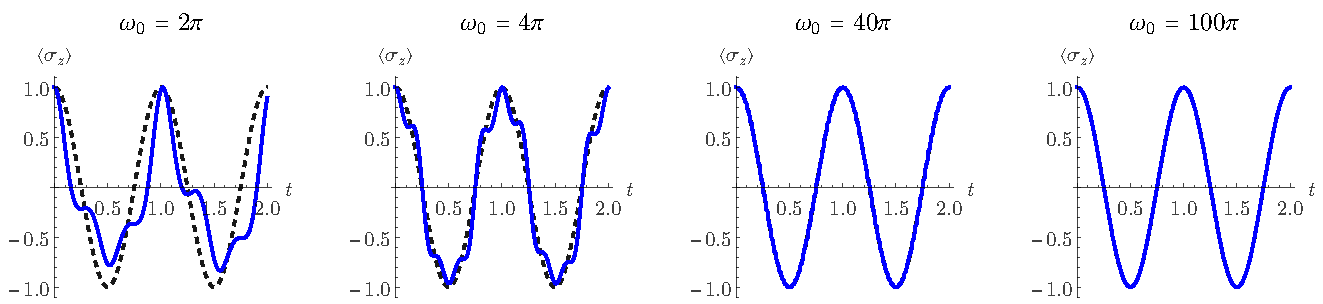
\includegraphics[width=1.0\textwidth]{figs/p23_1.pdf}
    \caption{Comparison of the exact solution (black) and the solution in the rotating wave approximation (blue).}
    \label{fig:rwa}
\end{figure}


We could find solution in general case $\delta \neq 0$ in RWA:
\begin{equation*}
	\langle \sigma_z\rangle(t) = \cos (\Omega_\delta t) + \frac{\delta ^2}{\delta ^2+\Omega ^2}(1-\cos (\Omega_\delta t )),
	\hspace{10 mm} 
	\Omega_\delta = \sqrt{\Omega^2 + \delta^2},
\end{equation*}
with general Rabi frequency $\Omega_\delta$. For different $\delta = 0, \Omega, 2 \Omega$ and $\Omega=2\pi$ we could compare different behaviour (fig. \ref{fig:rod}).

\begin{figure}[h]
    \centering
    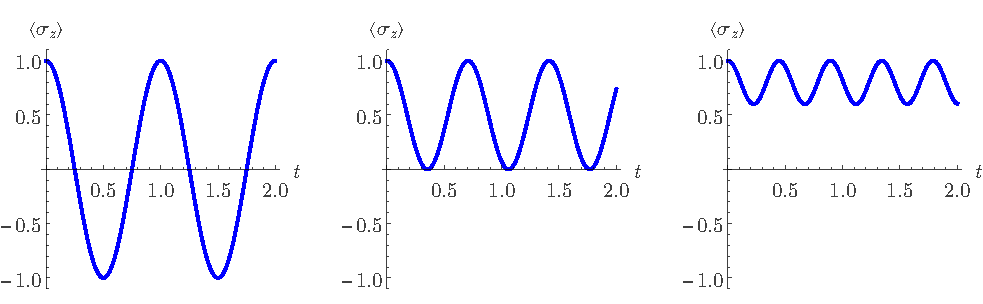
\includegraphics[width=0.75\textwidth]{figs/p23_2.pdf}
    \caption{Rabi oscillations at different detuning values}
    \label{fig:rod}
\end{figure}


\subsection{Dephasing and Decoherence in a TLS}

We could calculate $\langle \vc{\sigma}\rangle$, using  \eqref{leq}:
\begin{equation*}
	\rho(t) = \begin{pmatrix}
	    1-|\beta|^2 e^{- \Gamma_1 t} & \alpha \bar{\beta} e^{-\Gamma_2 t} \\
	    \bar{\alpha} \beta e^{- \Gamma_2 t} & |\beta|^2 e^{-\Gamma_1 t} \\
	\end{pmatrix},
	\hspace{0.5cm} \Rightarrow \hspace{0.5cm}
	\left.\begin{aligned}
	   \langle \sigma_x\rangle &= (\alpha \bar{\beta} + \bar{\alpha} \beta ) e^{- \Gamma_2 t}\\
	   \langle \sigma_y\rangle &= i(\alpha \bar{\beta} - \bar{\alpha} \beta ) e^{- \Gamma_2 t} \\
	   \langle \sigma_z\rangle &= 1 - 2 |\beta|^2 e^{-t \Gamma_1}
	\end{aligned}\right.
\end{equation*}
Substituting the initial state $\tfrac{1}{\sqrt{2}}\ket{0} + \tfrac{1}{\sqrt{2}}\ket{1}$
\begin{equation*}
	\langle \sigma_x\rangle =  e^{- \Gamma_2 t},
	\hspace{10 mm} 
	\langle \sigma_y\rangle = 0,
	\hspace{10 mm}
	\langle \sigma_z\rangle = 1 - e^{- \Gamma_1 t},
\end{equation*}
thus by measuring the various components we can find the $\Gamma_1$ and $\Gamma_2$, it's just exponential decay.


